\newpage
\subsection{Atomic Design Systems} \label{Atomic Design Systems}
% NOTE DONE: Add pictures of atoms, ... in use
This section will explore Atomic Design and its suitability for design and code collaboration. Web
designer Brad Frost introduced this design system methodology by drawing on chemistry to define a
hierarchical system.

\textbf{Atoms} \\
\begin{figure}[H]
	\centering
    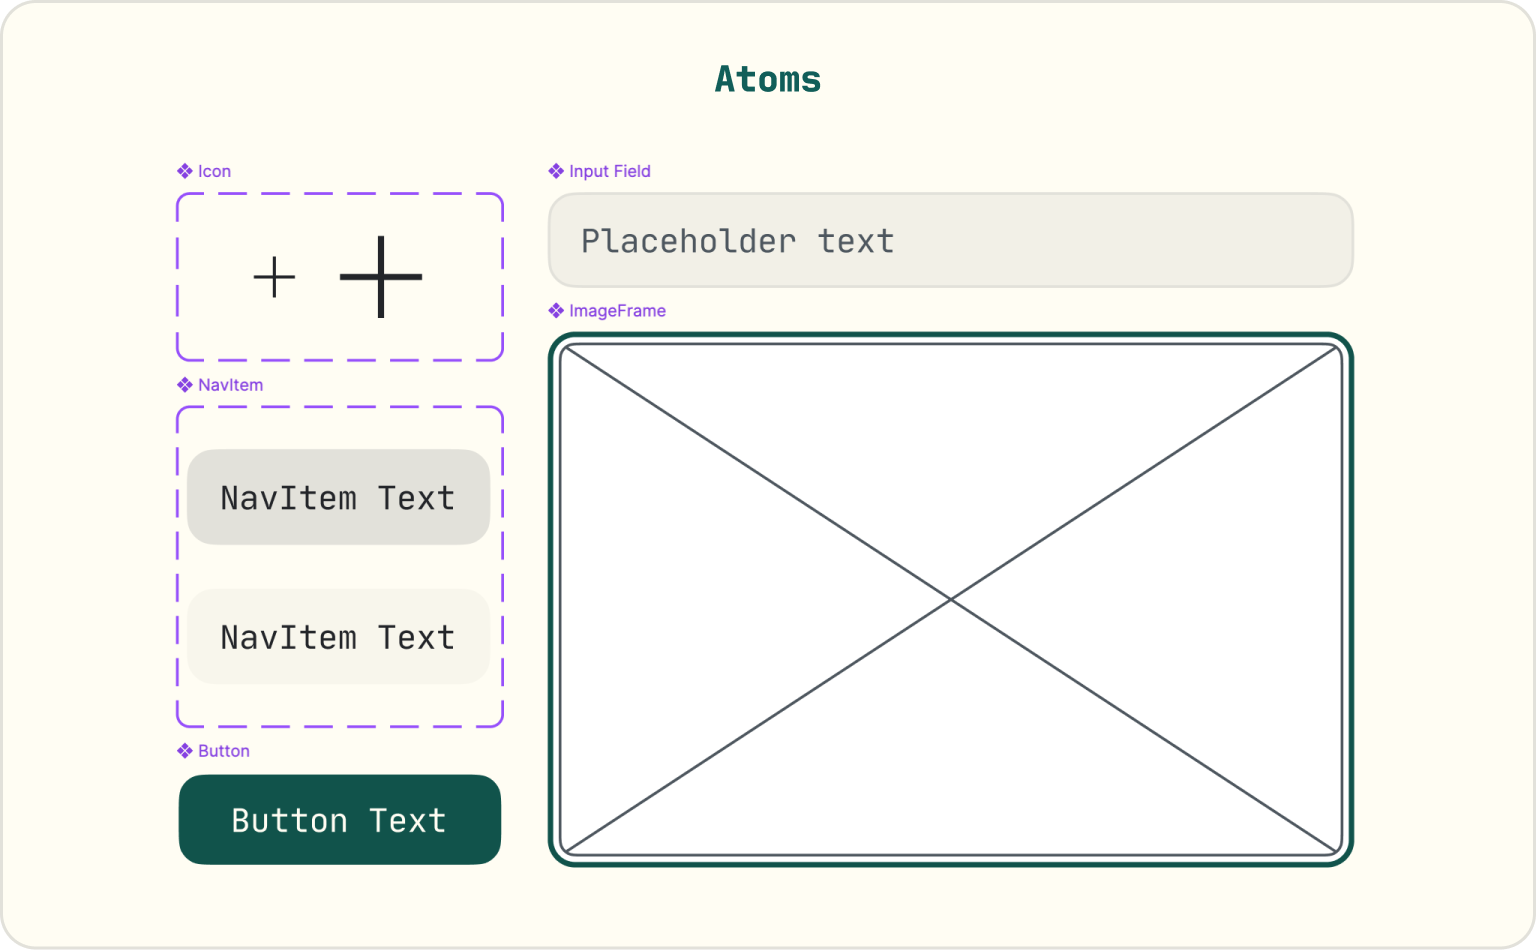
\includegraphics[width=250pt]{Chapter 2/Atoms.png}
    \caption{Atomic Design: Example of an Atoms (Source: own illustration)}
\end{figure}
Atoms are the smallest building blocks of the design. They are the basic elements like buttons,
textfields, colors, fonts or icons. Parts that cannot be broken down any further.
\vglcite[43,44]{frostAtomicDesign2016} 

\textbf{Molecules} \\
\begin{figure}[H]
	\centering
    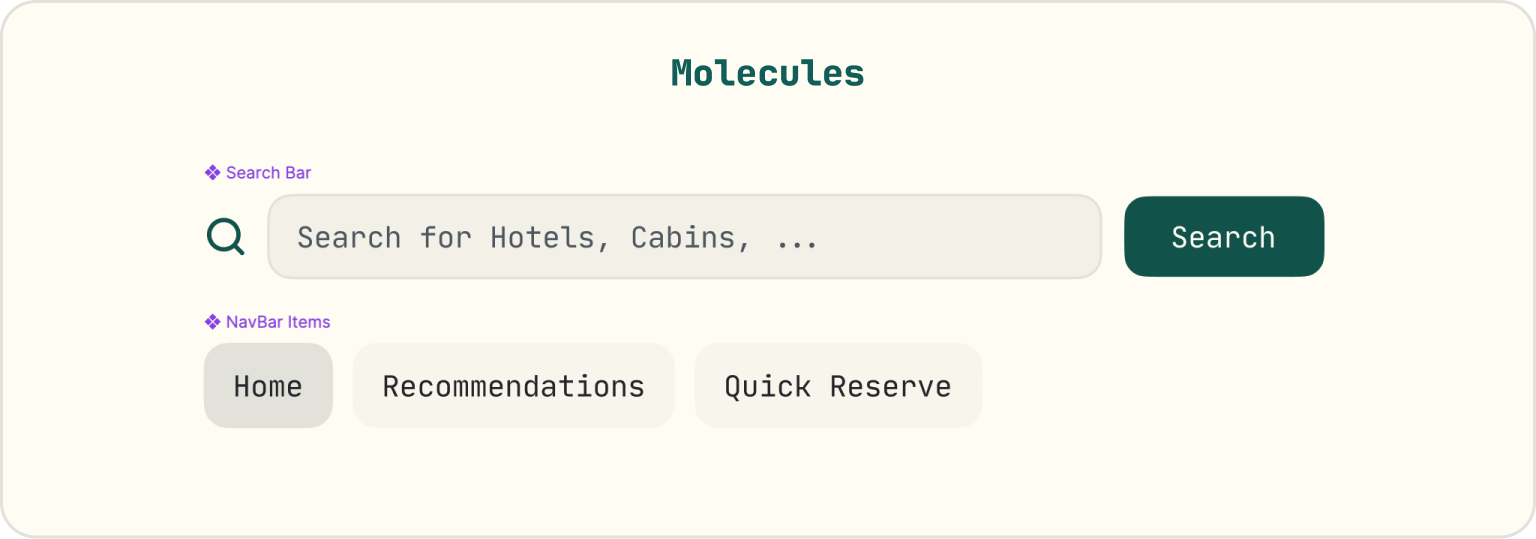
\includegraphics[width=250pt]{Chapter 2/Molecules.png}
    \caption{Atomic Design: Example of Molecules (Source: own illustration)}
\end{figure}
Molecules are groups of Atoms that together form a simple group of UI. For example, combining
a headline, an icon and filter buttons it would form a neat filter or navigation bar. Abstract Atoms
assemble to have a purpose. \vglcite[44,45]{frostAtomicDesign2016} 

\textbf{Organisms} \\
\begin{figure}[H]
	\centering
    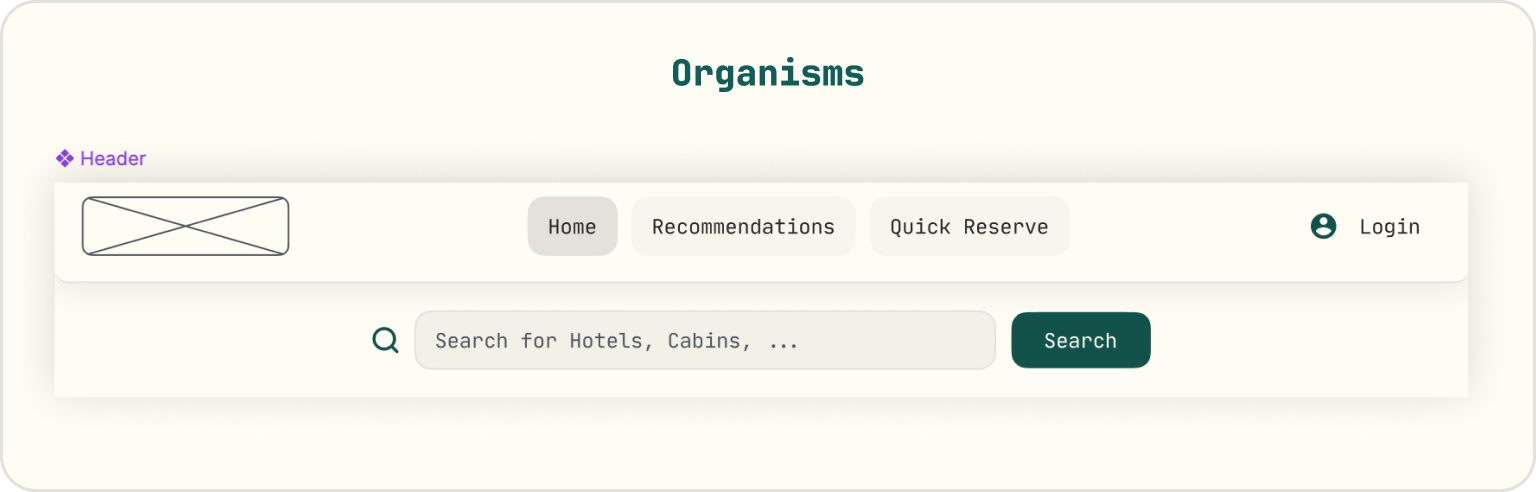
\includegraphics[width=250pt]{Chapter 2/Organisms.png}
    \caption{Atomic Design: Example of an Organism (Source: own illustration)}
\end{figure}
Organisms are more complex groups of UI elements. They can be a combination of Atoms, Molecules and
also other Organisms. When combining the bar Molecules, a few buttons and an image Atom, it would
form a functional booking service header. \vglcite[46,48]{frostAtomicDesign2016}

\textbf{Templates} \\
\begin{figure}[H]
	\centering
    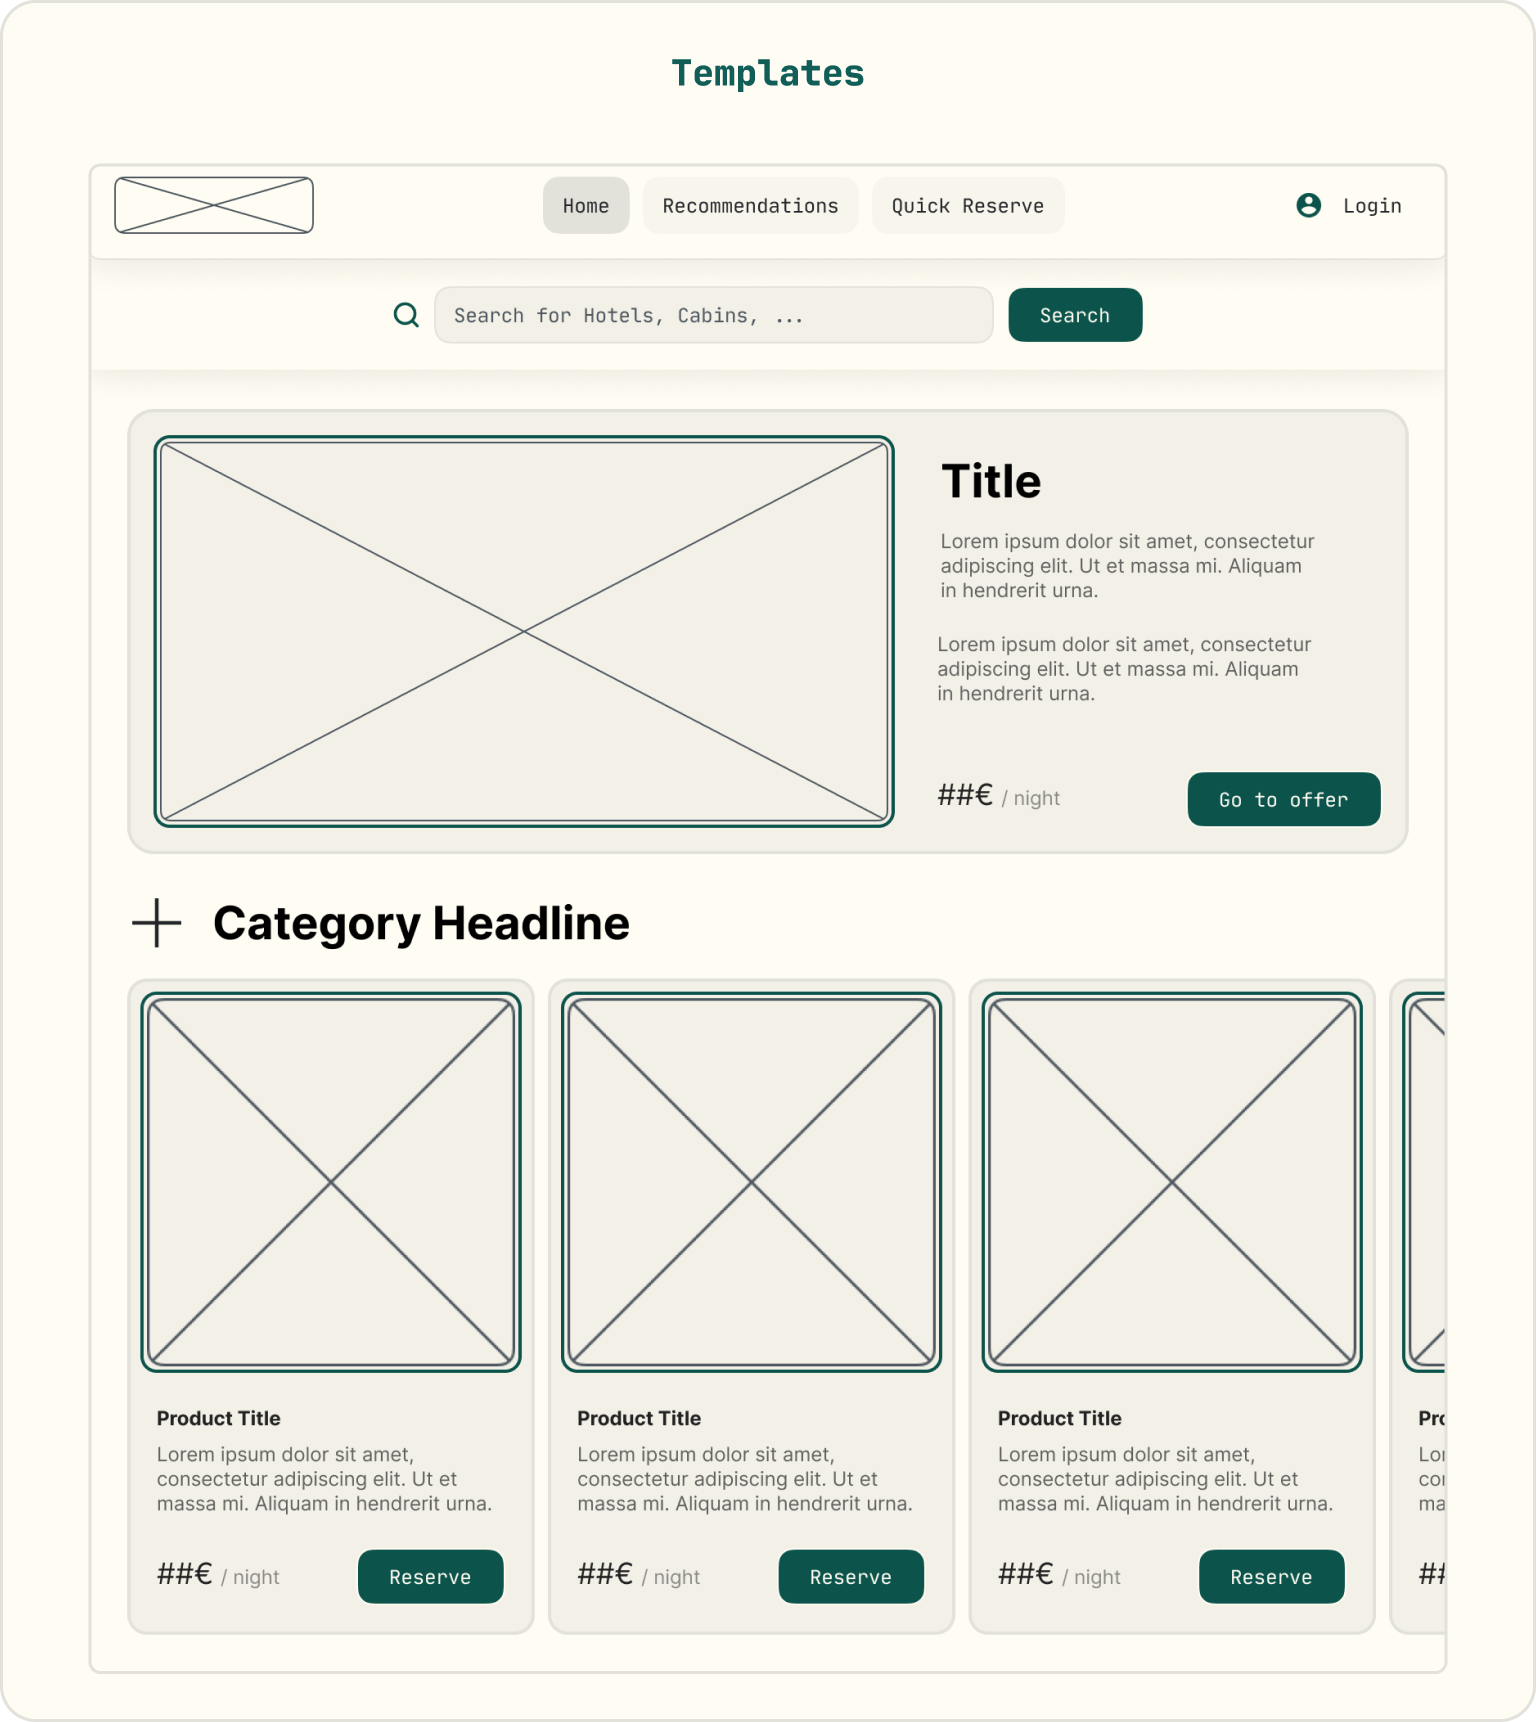
\includegraphics[width=250pt]{Chapter 2/Templates.png}
    \caption{Atomic Design: Example of a Template (Source: own illustration)}
\end{figure}
Templates are like blueprints of pages. They consist of Organisms and Molecules and define the
layout of a page, giving actual meaning to the UI elements. It shows the thought out content
structure, without any real content. \vglcite[48,51]{frostAtomicDesign2016}

\textbf{Pages}\\
\begin{figure}[H]
	\centering
    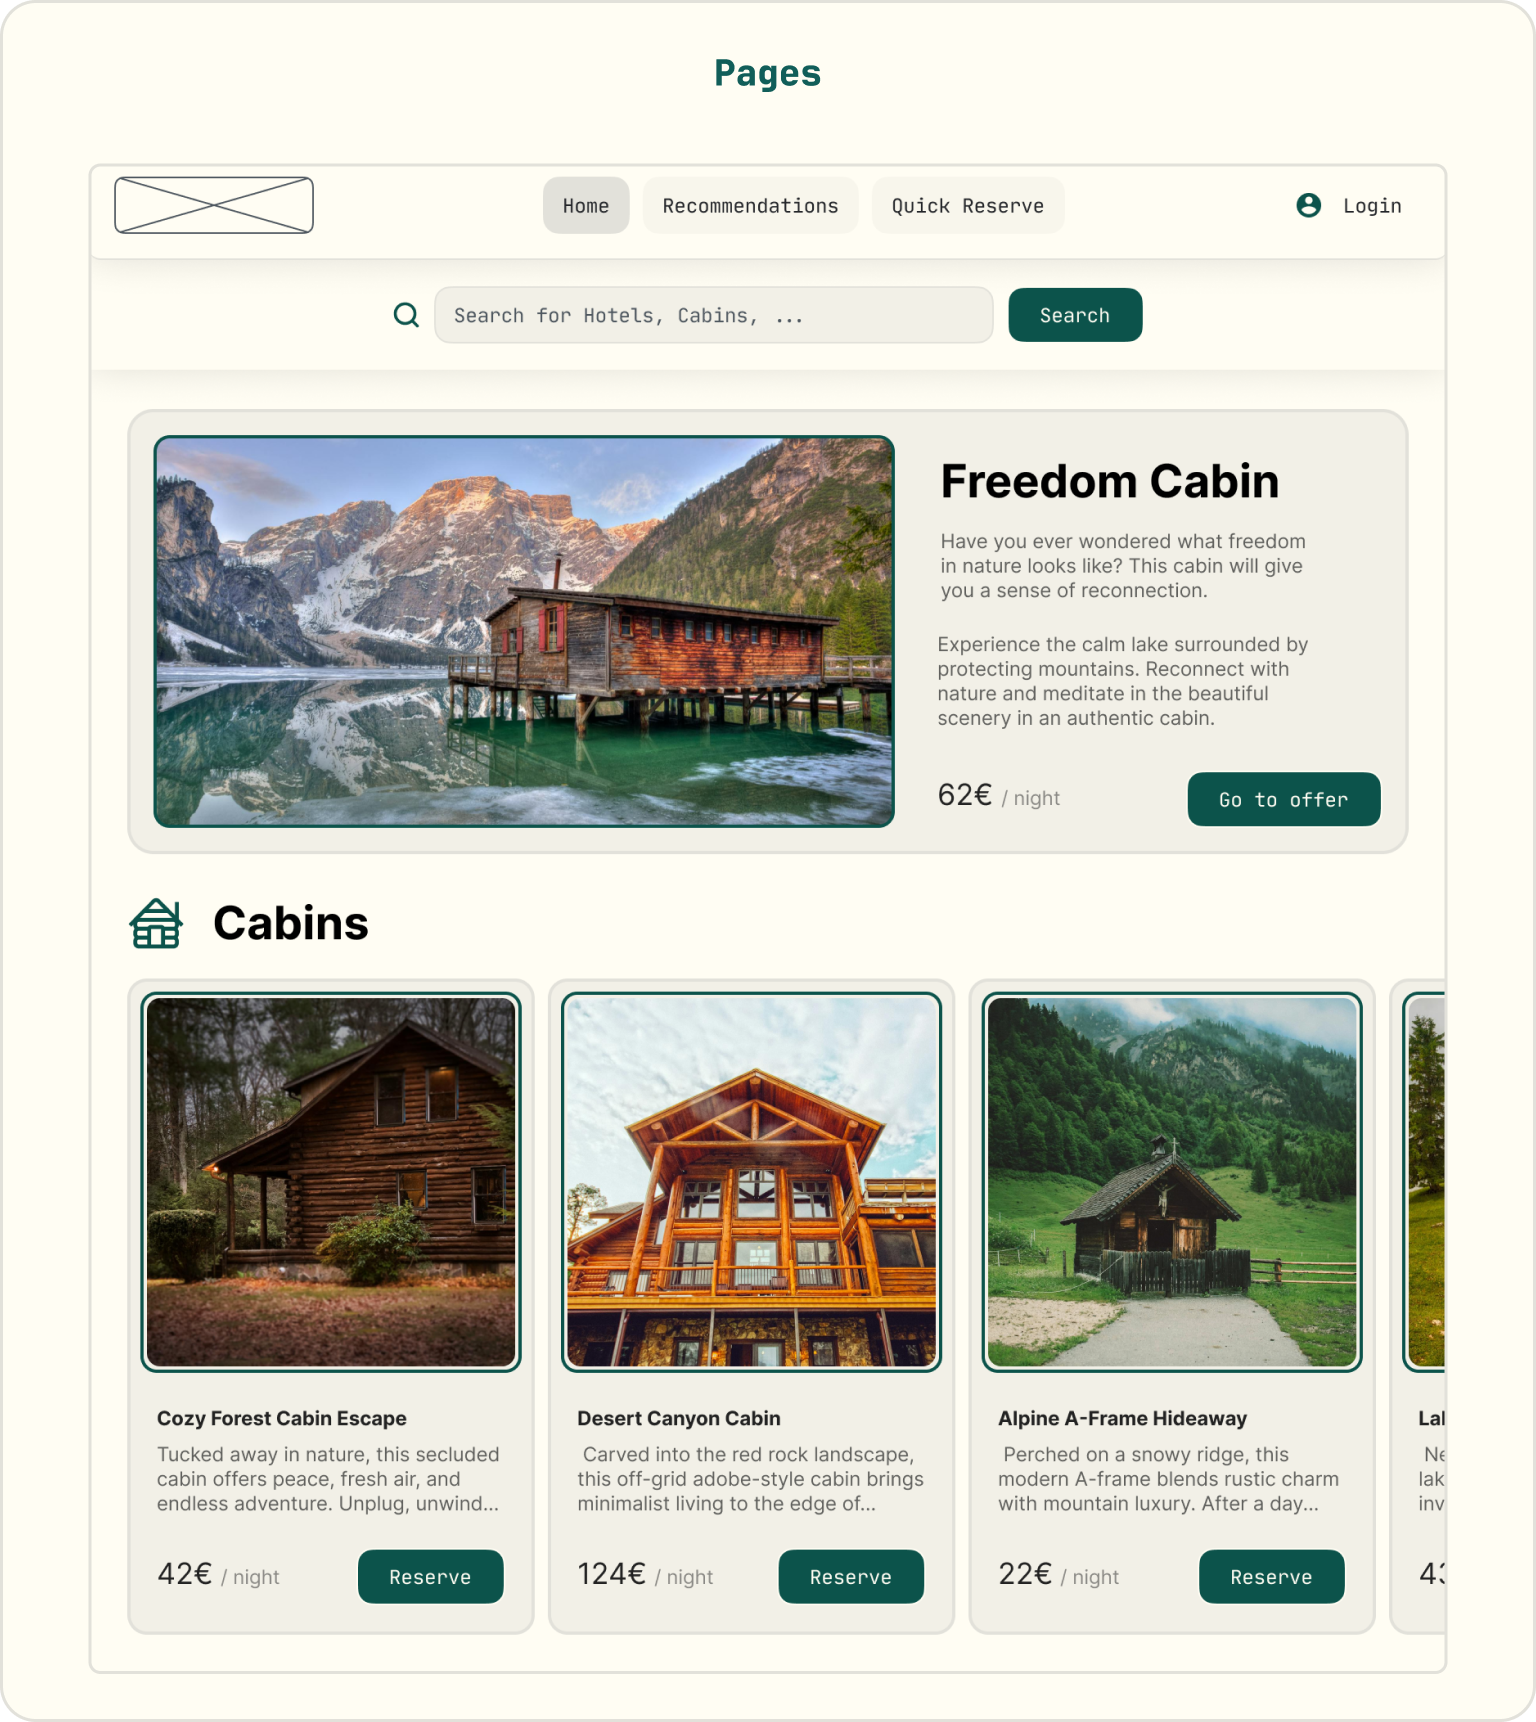
\includegraphics[width=250pt]{Chapter 2/Pages.png}
    \caption{Atomic Design: Example of a Page (Source: own illustration)}
\end{figure}
Pages take Templates as a basis and fill them with actual content. These represent how the final
delivered product will or should look like. \vglcite[52,55]{frostAtomicDesign2016}

Picturing this methodology as building with Lego often helps improve understanding. Atoms can be
seen as individual Lego bricks which cannot be made any smaller. These bricks can be stacked
together creating bigger more complex builds. By using these defined pieces, a Lego world can be
constructed that always looks consistent, but is still flexible enough to build anything.

While this analogy seems simple, it is actually quite powerful, since it demonstrates exactly what
we want from design systems. Having a set of clearly defined rules. Rules which give both designers
and engineers the time to actually focus on solving user needs without concerns about the design
getting inconsistent or feeling too constrained. \vglcite[13]{vesselovBuildingDesignSystems2019}

\subsubsection{Advantages and Drawbacks}
Having such a hierarchical component based design system has major advantages. However, it also
comes with several drawbacks. In order to tackle these challenges, it is essential to know what to
look out for.

\begin{itemize}
	\item Advantages
	      \begin{description}
		      \item[Support iterative workflows] - Working with Atomic Design supports an iterative
		            workflow. You can start with the smallest elements, build up a number of
		            definitions, then take a step back to look at how they work together. As soon as
		            something is not working together, the smaller elements can be adjusted. Having
		            this flexibility, while still having a clear structure, working iteratively
		            becomes much easier. \vglcite[57]{frostAtomicDesign2016}
		      \item[Changing it once, changes it everywhere] - When noticing that the padding
		            of a button is too small, it can be changed in the button definition and every
		            button across the whole design system using this definition will be updated.
		            This way, a tedious redo of everything is avoided, since there is always one
		            source of truth.
		      \item[Opportunity to work as close with devs as possible] - As already mentioned
		            before, the structure of the system is very close to how devs actually work.
		            Integrating this hierarchical, component-based system into the design process
		            from the start should, in theory, naturally streamline collaboration and make
		            the handoff between design and development much smoother.

		            \begin{figure}[h!]
			            \begin{center}
				            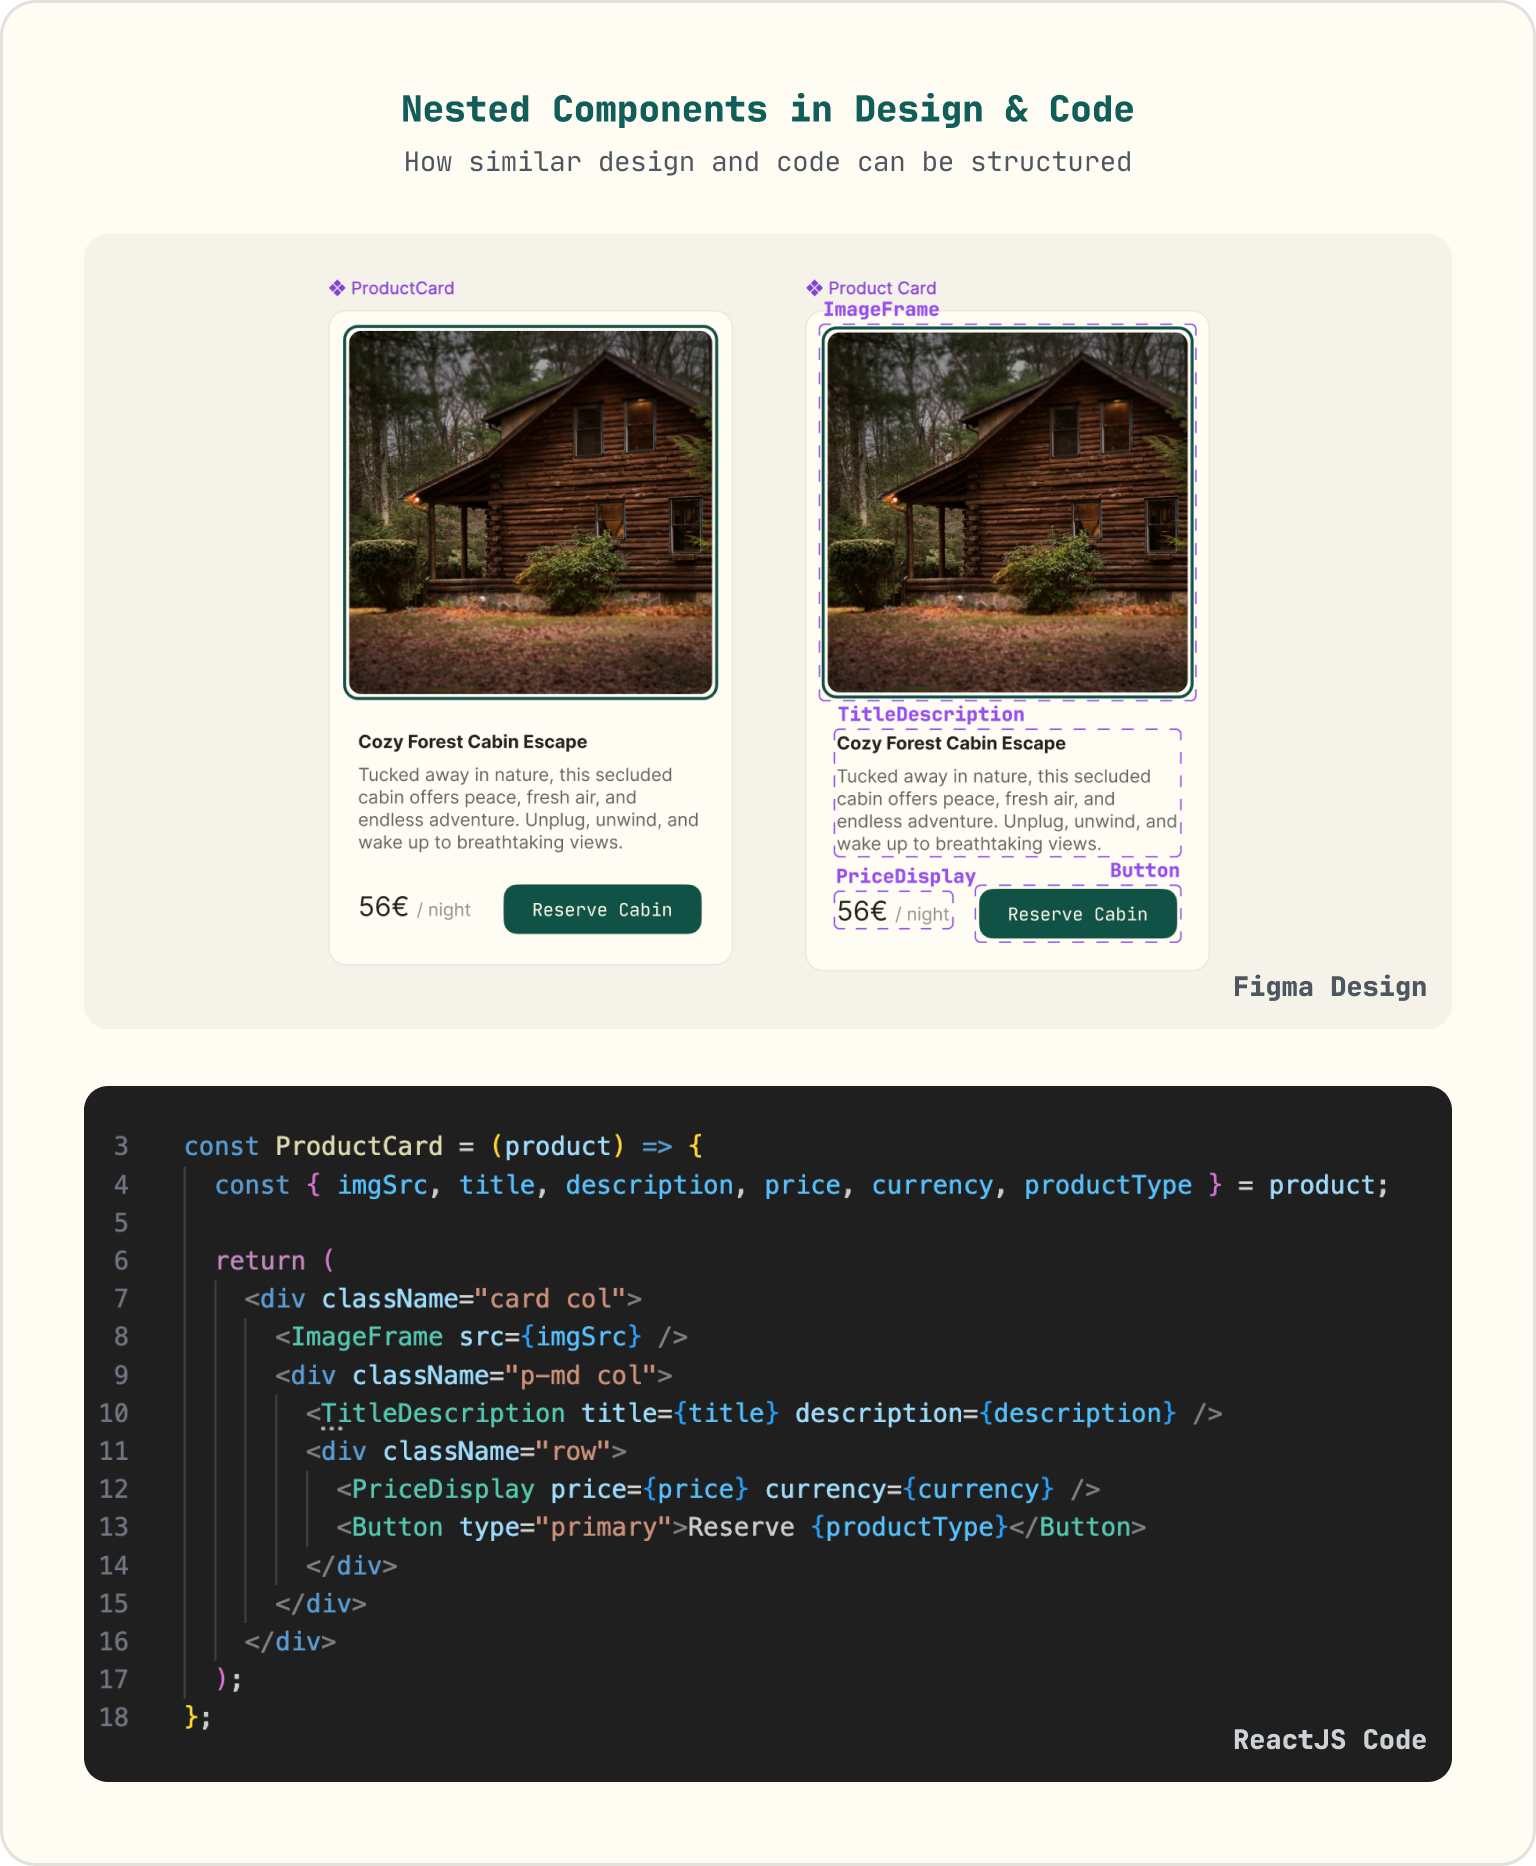
\includegraphics[width=300pt, height=\textheight,keepaspectratio]{Chapter 2/CodeDesign Similarity.png}
				            \caption{Similarity of design and code implementation (Source: own illustration)}
			            \end{center}
		            \end{figure}
		            ^^ Sample image showing how similar the design and code can be in terms of structure
		            % NOTE DONE: Add graphics UI Design and Developed Code and how similar it can be
	      \end{description}
	\item Drawbacks
	      \begin{description}
		      \item[Confusion about nomenclature] - Some teams struggle with the abstract terms of
		            Atomic Design and have a hard time assigning components to the right category.
		            As an example, the team at Bridge Studio for example, decided to use different
		            terms like "Foundations" or "Components" to make it easier to group and
		            understand the elements. However, they still kept the mindset of Atomic Design.
		            \vglcite{jamesecclestonWhatsWrongAtomic2021}

		            Brad Frost actively encourages teams to adapt the system to their needs, by
		            keeping the core principles in mind and altering the notations for example.
		            \vglcite[59]{frostAtomicDesign2016}
		      \item[Feeling too restricted] - When working with a design system, it often feels like
		            it hinders creativity. It definitely can, if not used correctly. It is important
		            to remember that it is a tool to help, not restrict. As the product, the design
		            system is intended for, evolves iteratively, so should the design system.
		            \vglcite[106]{vesselovBuildingDesignSystems2019}
	      \end{description}
\end{itemize}

% \subsubsection{Common Best Practices}
% Basically say that naming should be clear but not too specific, Using Figma features for design tokens such as variables and styles. Not overdoing it right
% from the start cite: Sarah Vesselov's book page 21
% Think of it as a process iteratively evolving over time like the product it is used for. The Design
% System is never a finished product.
% https://uxdesign.cc/to-create-an-excellent-design-system-treat-it-like-a-collaborative-process-6602376bfef6
